\documentclass[a4paper]{article}
\usepackage{amssymb,amsmath,amsthm,amsfonts}
\usepackage{mathtools}
\usepackage{multicol,multirow}
\usepackage{calc}
\usepackage{enumerate,float,graphics,graphicx}
\usepackage{ifthen}
\usepackage{setspace}
\usepackage[dvipsnames]{xcolor}
\usepackage{subfig}
\usepackage[landscape]{geometry}
\usepackage[colorlinks=true,citecolor=blue,linkcolor=blue]{hyperref}


\ifthenelse{\lengthtest { \paperwidth = 11in}}
    { \geometry{top=.5in,left=.5in,right=.5in,bottom=.5in} }
	{\ifthenelse{ \lengthtest{ \paperwidth = 297mm}}
		{\geometry{top=1cm,left=1cm,right=1cm,bottom=1cm} }
		{\geometry{top=1cm,left=1cm,right=1cm,bottom=1cm} }
	}

\pagestyle{empty}
\makeatletter
\renewcommand{\section}{\@startsection{section}{1}{0mm}%
                                {-1ex plus -.5ex minus -.2ex}%
                                {0.5ex plus .2ex}%x
                                {\normalfont\large\bfseries}}
\renewcommand{\subsection}{\@startsection{subsection}{2}{0mm}%
                                {-1explus -.5ex minus -.2ex}%
                                {0.5ex plus .2ex}%
                                {\normalfont\normalsize\bfseries}}
\renewcommand{\subsubsection}{\@startsection{subsubsection}{3}{0mm}%
                                {-1ex plus -.5ex minus -.2ex}%
                                {1ex plus .2ex}%
                                {\normalfont\small\bfseries}}
\makeatother
\setcounter{secnumdepth}{0}
\setlength{\parindent}{0pt}
\setlength{\parskip}{0pt plus 0.5ex}
% -----------------------------------------------------------------------

\title{Circuits-2 cheat sheet}
%\doublespacing
\begin{document}

\raggedright
\footnotesize

\begin{center}
     \Large{\textbf{EEC 221 - Circuits2 cheat sheet\footnote{ \textcolor{darkgray}{Taha Ahmed}}}} \\
\end{center}
\begin{multicols}{3}
\setlength{\premulticols}{1pt}
\setlength{\postmulticols}{1pt}
\setlength{\multicolsep}{1pt}
\setlength{\columnsep}{2pt}


\section{Transfer function}
$$\textbf{H}(\omega) = \frac{\textbf{Y}(\omega)}{\textbf{X}(\omega)}$$

\begin{align*}
\text{Voltage gain} &= \frac{\textbf{V}_o(\omega)}{\textbf{V}_i(\omega)}\\
\text{Current gain} &= \frac{\textbf{I}_o(\omega)}{\textbf{I}_i(\omega)}\\
\text{Transfer impedence} &= \frac{\textbf{V}_o(\omega)}{\textbf{I}_i(\omega)}\\
\text{Transfer admittance} &= \frac{•\textbf{I}_o(\omega)}{\textbf{V}_i(\omega)}
\end{align*}

For RC circuit: $\displaystyle \omega_0 = \frac{1}{RC}$
\vspace{5px}

For RL circuit: $\displaystyle \omega_0 = \frac{R}{L}$


\section{Resonance}
\subsection{Series resonance}
\begin{align*}
\omega_0 &= \frac{1}{\sqrt{LC}}\\
f_0 &= \frac{1}{2\pi \sqrt{LC}}\\
\end{align*}

at resonance:
\begin{align*}
Z=R &&\mid I \mid_{max} = \frac{\mid V \mid_{max}}{R} &&X_L=X_C
\end{align*}

The average power at RLC circuits:
$$P(\omega) = \frac{1}{2} I^2 R$$
The average power at resonance: 
$$P(\omega) = \frac{1}{2} I_{max}^2 R = \frac{1}{2} \frac{V_{max}^2}{R}$$

Half power frequencies:
\begin{align*}
&\omega_1 , \omega_2 = \mp \frac{R}{2L} + \sqrt{\left( \frac{R}{2L} \right)^2  + \frac{1}{LC} }\\
&\omega_0 = \sqrt{\omega_1 \omega_2}
\end{align*}

Bandwidth:
\begin{align*}
B = \omega_2 - \omega_1 = \frac{R}{L}
\end{align*}

Quality factor:
\begin{align*}
Q = \frac{\text{Peak energy}}{\text{Energy dissipated}} = \frac{\omega_0}{B}
\end{align*}

When $Q>10$ :
\begin{align*}
\omega_1 = \omega_0 - \frac{B}{2}\\
\omega_2 = \omega_0 + \frac{B}{2}\\
\end{align*}

\subsection{Parallel resonance}

\begin{align*}
\omega_0 &= \frac{1}{\sqrt{LC}}\\
f_0 &= \frac{1}{2\pi \sqrt{LC}}\\
\end{align*}

at resonance:
\begin{align*}
Z=R &&\mid I \mid_{max} = \frac{\mid V \mid_{max}}{R} &&X_L=X_C
\end{align*}

The average power at RLC circuits:
$$P(\omega) = \frac{1}{2} I^2 R$$
The average power at resonance: 
$$P(\omega) = \frac{1}{2} I_{max}^2 R = \frac{1}{2} \frac{V_{max}^2}{R}$$

Half power frequencies:
\begin{align*}
&\omega_1 , \omega_2 = \mp \frac{1}{2RC} + \sqrt{\left( \frac{1}{2RC} \right)^2  + \frac{1}{LC} }\\
&\omega_0 = \sqrt{\omega_1 \omega_2}
\end{align*}

Bandwidth:
\begin{align*}
B = \omega_2 - \omega_1 = \frac{1}{RC}
\end{align*}

Quality factor:
\begin{align*}
Q = \frac{\text{Peak energy}}{\text{Energy dissipated}} = \frac{\omega_0}{B}
\end{align*}

When $Q>10$ :
\begin{align*}
\omega_1 = \omega_0 - \frac{B}{2}\\
\omega_2 = \omega_0 + \frac{B}{2}\\
\end{align*}


\section*{Magnetically Coupled Circuits}

M (Mutual inductance):
\begin{align*}
M=K\sqrt{L_1 \, L_2} \tag{k: couppling coefficent}
\end{align*} 

Dot convention:
%\begin{figure}[H] 
%	\centering
%	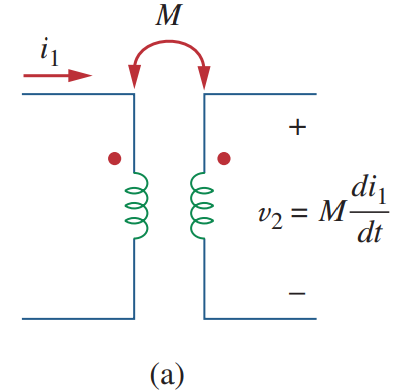
\includegraphics[width = 0.25\textwidth]{1}
%%	\caption{}
%	\label{fig:1}
%\end{figure}


\begin{figure}[H]
    \centering
    \subfloat{{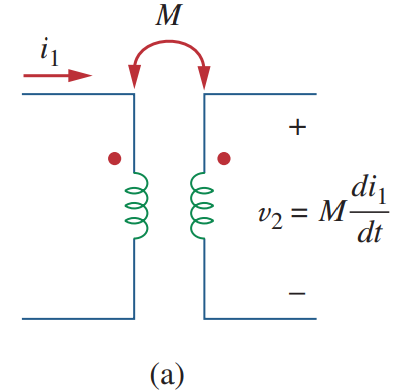
\includegraphics[width = 0.125\textwidth]{1}}}%
    \qquad
    \subfloat{{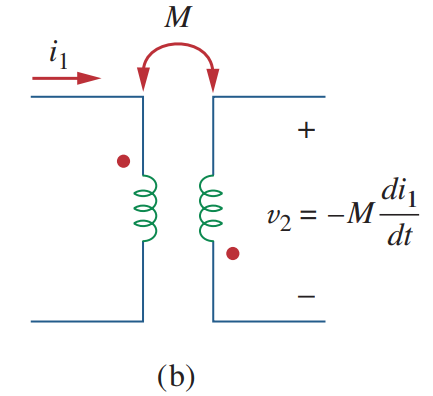
\includegraphics[width = 0.125\textwidth]{2} }}%
%    \caption{2 Figures side by side}%
    \label{fig:example}%
\end{figure}

\begin{figure}[H]
    \centering
    \subfloat{{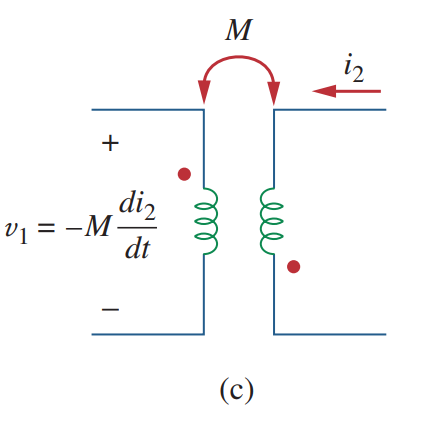
\includegraphics[width = 0.125\textwidth]{3}}}%
    \qquad
    \subfloat{{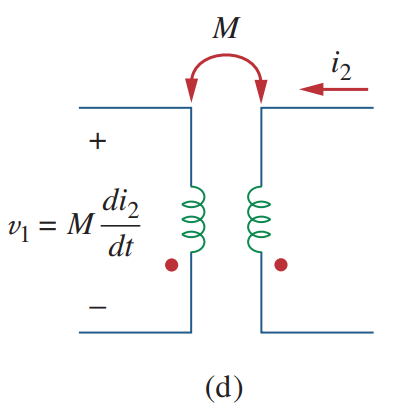
\includegraphics[width = 0.125\textwidth]{4} }}%
%    \caption{2 Figures side by side}%
    \label{fig:example}%
\end{figure}

Dependent source representation:

\begin{figure}[H]
    \centering
    \subfloat{{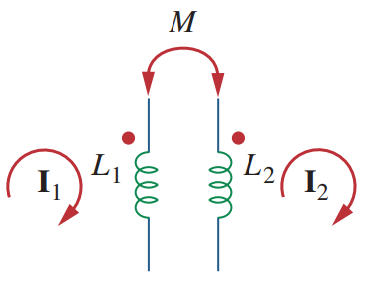
\includegraphics[width = 0.125\textwidth]{dsr1}}}%
    \qquad
    \subfloat{{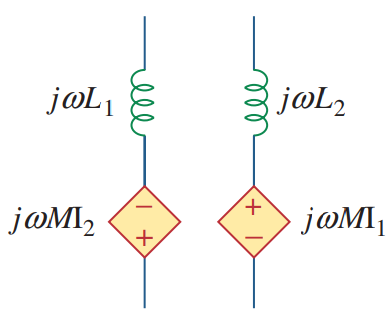
\includegraphics[width = 0.125\textwidth]{dsr2} }}%
%    \caption{2 Figures side by side}%
    \label{fig:example}%
\end{figure}

Series-aiding connection:
$$l_{eq}=L_1+L_2+2M$$

\begin{figure}[H] 
	\centering
	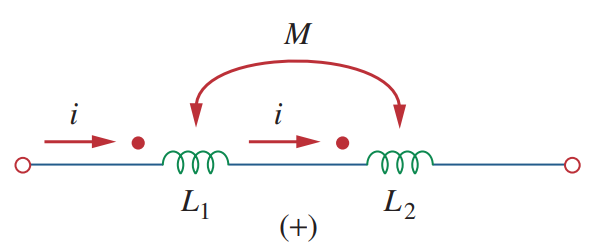
\includegraphics[width = 0.2\textwidth]{5}
%	\caption{}
	\label{fig:1}
\end{figure}

Series-opposing connection:
$$l_{eq}=L_1+L_2-2M$$

\begin{figure}[H] 
	\centering
	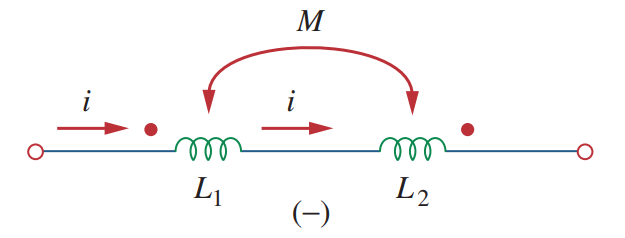
\includegraphics[width = 0.2\textwidth]{6}
%	\caption{}
	\label{fig:1}
\end{figure}


Energy stored:
\begin{align*}
W = \frac{1}{2}L_1 I_1^2 + \frac{1}{2}L_2 I_2^2 + MI_1 I_2 \tag{two currents enter the dots or leave}\\
W = \frac{1}{2}L_1 I_1^2 + \frac{1}{2}L_2 I_2^2 - MI_1 I_2 \tag{one enters, one leaves}
\end{align*}

Power dissipated in a resistor:
\begin{align*}
P &= |I_{RMS}|^2 \, R \tag{$I_{RMS} = \dfrac{I_{peak}}{\sqrt{2}}$}\\
P &= \frac{1}{2}|I_{peak}|^2 \, R
\end{align*} 


T model:
\begin{figure}[H] 
	\centering
	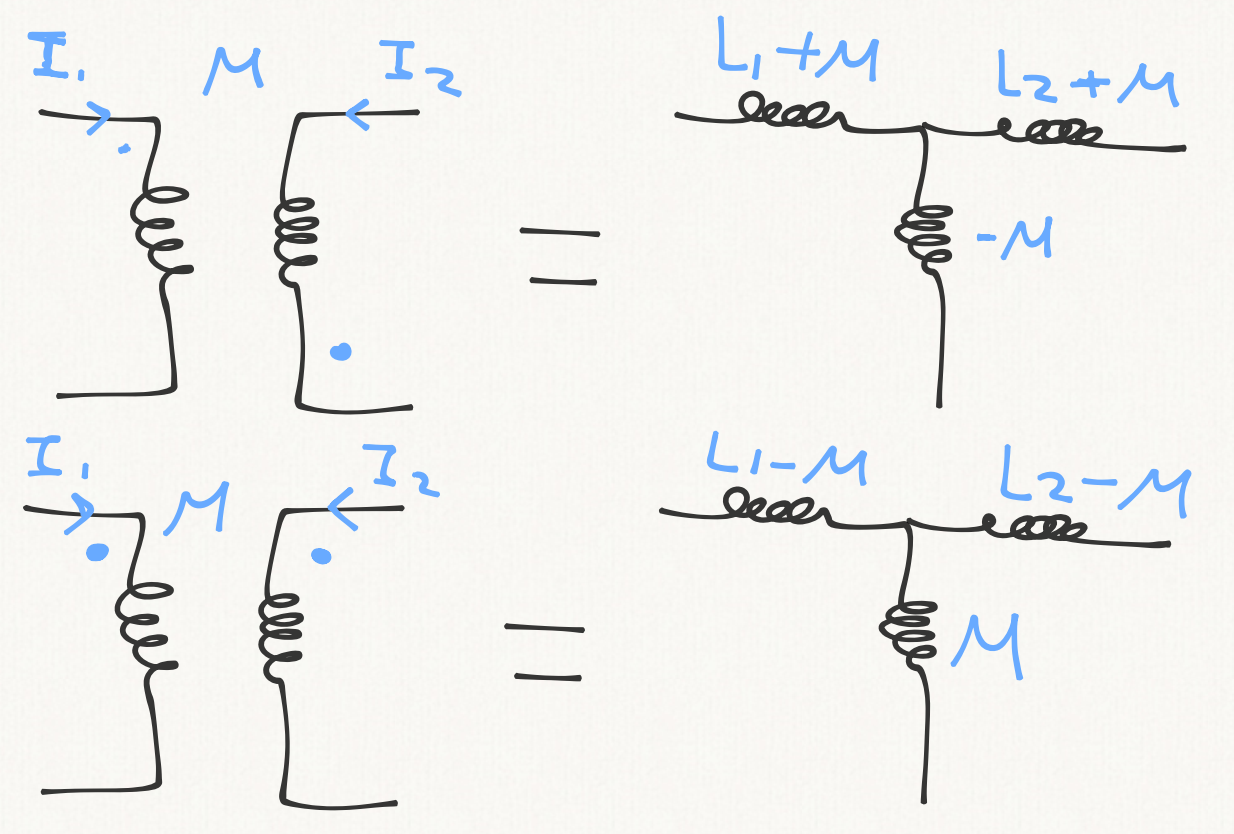
\includegraphics[width = 0.28\textwidth]{T}
%	\caption{}
	\label{fig:1}
\end{figure}

$\pi$ model:


\begin{figure}[H] 
	\centering
	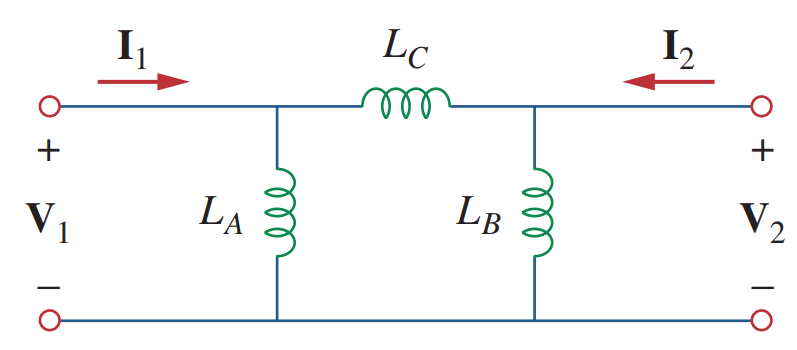
\includegraphics[width = 0.2\textwidth]{pi model}
%	\caption{}
	\label{fig:1}
\end{figure}

\begin{align*}
L_A &= \frac{L_1L_2 - M^2}{L_2 - M} &&L_B &= \frac{L_1L_2 - M^2}{L_1 - M}\\
L_C &= \frac{L_1L_2 - M^2}{M}
\end{align*}


\section{Transformer}
\subsection{Linear transformer $0 < k < 1$}


\begin{figure}[H] 
	\centering
	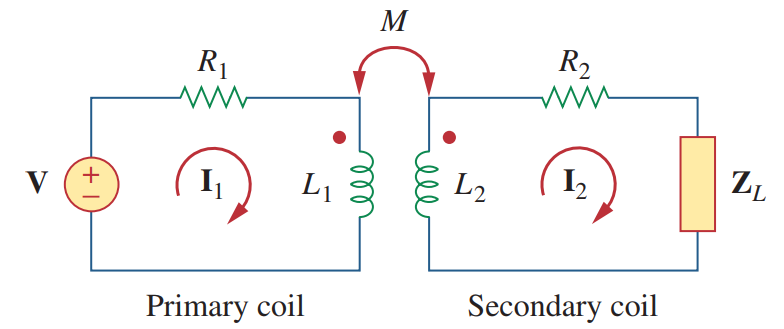
\includegraphics[width = 0.2\textwidth]{linear transformer}
%	\caption{}
	\label{fig:1}
\end{figure}

\begin{align*}
Z_{in}  &= R_1 +j\omega L_1 + \underbrace{\;\frac{\omega^2 M^2}{R_2 +j\omega L_2 + Z_L}\;}_{\text{reflected impedence}}= \frac{V}{I_1}\\
Z_{th}  &= R_2 +j\omega L_2 + \underbrace{\;\frac{\omega^2 M^2}{R_1 +j\omega L_1 
}\;}_{\text{reflected impedence}}
\end{align*}

for maximum power transfer:
$$ Z_L = Z_{th}^* $$

for maximum power transfer if $R_L$ is pure resistive:
$$ R_L = |Z_{th}| $$

\subsection{Ideal transformer k = 1}

\begin{align*}
n = \frac{N_2}{N_1} \tag{turns ratio}\\
\frac{V_2}{V_1} = n\\
\frac{I_2}{I_1} = \frac{1}{n}\\
\end{align*}

\begin{multicols}{2}
Referring from secondary to primary:
\begin{align*}
V_1' = \frac{V_2}{n} \\
I_1' = nI_2\\
Z_1' = \frac{V_2}{n^2}\\
\end{align*}
Referring from primary to secondary:
\begin{align*}
V_2' = n V_1 \\
I_2' = \frac{I_1}{n}\\
Z_2' = n^2 Z_1\\
\end{align*}
\end{multicols}

Sign roles:

if both voltages are +ve or -ve relative to the dotted terminals $\rightarrow$ use $+n$\\otherwise use $-n$

if both currents enter or leave the  dotted terminals $\rightarrow$ use $-n$\\otherwise use $+n$


\begin{figure}[H]
    \centering
    \subfloat{{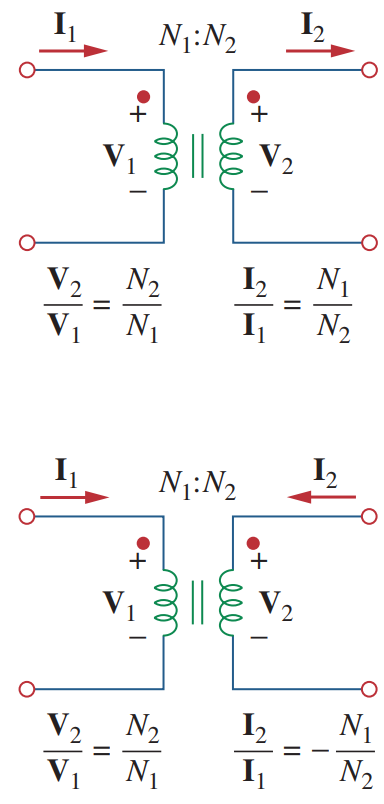
\includegraphics[width = 0.125\textwidth]{ideal1}}}%
    \qquad
    \subfloat{{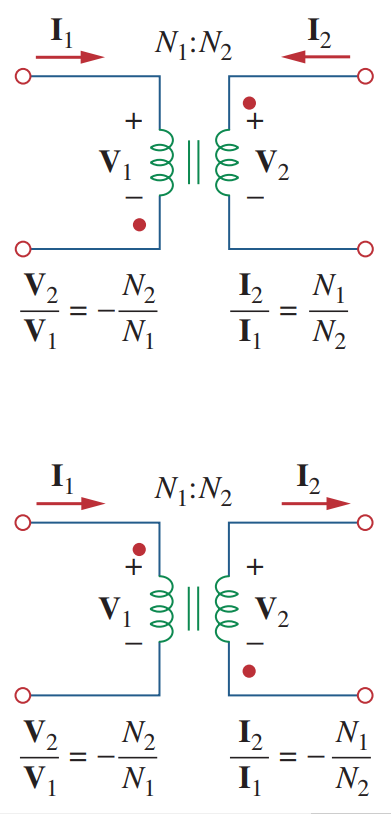
\includegraphics[width = 0.125\textwidth]{ideal2} }}%
%    \caption{2 Figures side by side}%
    \label{fig:example}%
\end{figure}

Complex power:
\begin{align*}
s_1 = V_1 I_1^*\\
s_2 = V_2 I_2^*\\
\boxed{s_1 = s_2}
\end{align*}

\subsection*{Ideal autotransformer}

\begin{figure}[H] 
	\centering
	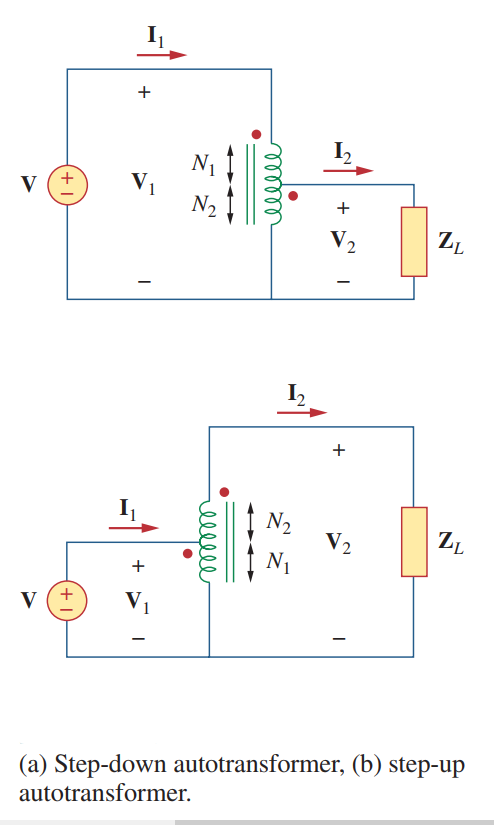
\includegraphics[width = 0.2\textwidth]{auto}
%	\caption{}
	\label{fig:1}
\end{figure}


Step down autotransformer:
\begin{align*}
\frac{V_1}{V_2} = \frac{N_1 + N_2}{N_2} \\
\\
\frac{I_1}{I_2} = \frac{N_2}{N_1 + N_2} 
\end{align*}

Step down autotransformer:
\begin{align*}
\frac{V_1}{V_2} = \frac{N_1 }{N_1 + N_2} \\
\\
\frac{I_1}{I_2} = \frac{N_1 + N_2}{N_1} 
\end{align*}

\section{Two port network}
\subsection{Impedance parameters [Z]}

$$
\begin{bmatrix}
V_1 \\
V_2 
\end{bmatrix}
=
\begin{bmatrix}
Z_{11} & Z_{12} \\
Z_{21} & Z_{22} 
\end{bmatrix}
\begin{bmatrix}
I_1 \\
I_2 
\end{bmatrix}
$$
\begin{align*}
V_1 = Z_{11}I_1 + Z_{12}I_2\\
V_2 = Z_{21}I_1 + Z_{22}I_2\\
\end{align*}
\begin{align*}
Z_{11} = \left. \frac{V_1}{I_1} \right|_{I_2 = 0} &&Z_{12} = \left. \frac{V_1}{I_2} \right|_{I_1 = 0}\\
Z_{21} = \left. \frac{V_2}{I_1} \right|_{I_2 = 0} &&Z_{22} = \left. \frac{V_2}{I_2} \right|_{I_1 = 0}
\end{align*}
for any T network:


\begin{figure}[H] 
	\centering
	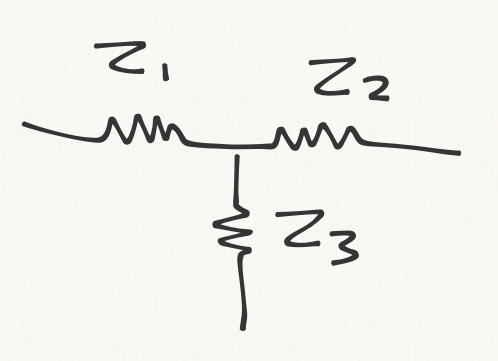
\includegraphics[width = 0.2\textwidth]{T p}
%	\caption{}
	\label{fig:1}
\end{figure}

\begin{align*}
Z = \begin{bmatrix}
Z_{1}+Z_{3} & Z_{3} \\
Z_{3} & Z{2}+Z_{3} 
\end{bmatrix}
\end{align*}

if $Z_{11} = Z_{22} \rightarrow$ symmetrical network\\
if $Z_{12} = Z_{21} \text{and has no dependent sources} \rightarrow$ reciprocal network

\subsection{Admittance parameters [y]}


$$
\begin{bmatrix}
I_1 \\
I_2 
\end{bmatrix}
=
\begin{bmatrix}
y_{11} & y_{12} \\
y_{21} & y_{22} 
\end{bmatrix}
\begin{bmatrix}
V_1 \\
V_2 
\end{bmatrix}
$$
\begin{align*}
I_1 = y_{11}V_1 + y_{12}V_2\\
I_2 = y_{21}V_1 + y_{22}V_2\\
\end{align*}
\begin{align*}
y_{11} = \left. \frac{I_1}{V_1} \right|_{I_2 = 0} &&y_{12} = \left. \frac{I_1}{V_2} \right|_{V_1 = 0}\\
y_{21} = \left. \frac{I_2}{V_1} \right|_{V_2 = 0} &&y_{22} = \left. \frac{I_2}{V_2} \right|_{V_1 = 0}
\end{align*}

for any T network:


\begin{figure}[H] 
	\centering
	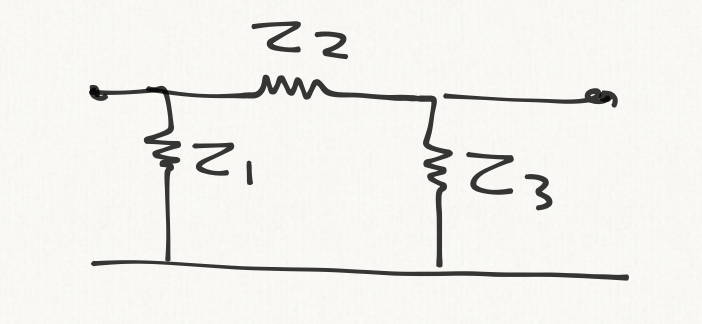
\includegraphics[width = 0.2\textwidth]{pi p}
%	\caption{}
	\label{fig:1}
\end{figure}

\begin{align*}
y = \begin{bmatrix}
 \frac{1}{Z_1} + \frac{1}{Z_2} & \frac{-1}{Z_2} \\
 \frac{-1}{Z_2} &  \frac{1}{Z_2} + \frac{1}{Z_3}
\end{bmatrix}
\end{align*}

note that $$[Z] = [y]^{-1}$$

remember $\rightarrow$ Let
\[
A = \begin{bmatrix}
       a_{11} & a_{12} \\ 
       a_{21} & a_{22}
    \end{bmatrix}
\]
be a full-rank $2\times2$ matrix. 
Then $\det A\equiv\lvert A\rvert=a_{11}a_{22}-a_{12}a_{21}\ne0$ and 
\[
A^{-1}=\begin{bmatrix}
          a_{11} & a_{12} \\ 
          a_{21} & a_{22}
       \end{bmatrix}^{-1}
      =\frac{1}{\lvert A\rvert}
       \begin{bmatrix*}[r]
           a_{22} & -a_{12} \\ 
          -a_{21} &  a_{11}
       \end{bmatrix*} \,.
\]

\subsection{Hybrid parameters [h]}



$$
\begin{bmatrix}
V_1 \\
I_2 
\end{bmatrix}
=
\begin{bmatrix}
h_{11} & h_{12} \\
h_{21} & h_{22} 
\end{bmatrix}
\begin{bmatrix}
I_1 \\
V_2 
\end{bmatrix}
$$
\begin{align*}
V_1 = h_{11}I_1 + h_{12}V_2\\
I_2 = h_{21}I_1 + h_{22}V_2\\
\end{align*}
\begin{align*}
h_{11} = \left. \frac{V_1}{I_1} \right|_{V_2 = 0} &&h_{12} = \left. \frac{V_1}{V_2} \right|_{I_1 = 0}\\
h_{21} = \left. \frac{I_2}{I_1} \right|_{V_2 = 0} &&h_{22} = \left. \frac{I_2}{V_2} \right|_{I_1 = 0}
\end{align*}

\subsection{Inverse Hybrid parameters [g]}



$$
\begin{bmatrix}
I_1 \\
V_2 
\end{bmatrix}
=
\begin{bmatrix}
g_{11} & g_{12} \\
g_{21} & g_{22} 
\end{bmatrix}
\begin{bmatrix}
V_1 \\
I_2 
\end{bmatrix}
$$
\begin{align*}
I_1 = g_{11}V_1 + g_{12}I_2\\
V_2 = g_{21}V_1 + g_{22}I_2\\
\end{align*}
\begin{align*}
g_{11} = \left. \frac{I_1}{V_1} \right|_{I_2 = 0} &&g_{12} = \left. \frac{I_1}{I_2} \right|_{V_1 = 0}\\
g_{21} = \left. \frac{V_2}{V_1} \right|_{I_2 = 0} &&g_{22} = \left. \frac{V_2}{I_2} \right|_{V_1 = 0}
\end{align*}

note that $$[g] = [h]^{-1}$$

\subsection{Transmission parameters [T]}



$$
\begin{bmatrix}
V_1 \\
I_1 
\end{bmatrix}
=
\begin{bmatrix}
A & B \\
C & D 
\end{bmatrix}
\begin{bmatrix}
V_2 \\
-I_2 
\end{bmatrix}
$$
\begin{align*}
V_1 = AV_2 - BI_2\\
I_1 = CV_2 - DI_2\\
\end{align*}
\begin{align*}
A = \left. \frac{V_1}{V_2} \right|_{I_2 = 0} &&B = \left. \frac{-V_1}{I_2} \right|_{V_2 = 0}\\
C = \left. \frac{I_2}{V_2} \right|_{I_2 = 0} &&D = \left. \frac{I_1}{I_2} \right|_{V_1 = 0}
\end{align*}


\subsection{Inverse transmission parameters [t]}



$$
\begin{bmatrix}
V_2 \\
I_2 
\end{bmatrix}
=
\begin{bmatrix}
a & b \\
c & d 
\end{bmatrix}
\begin{bmatrix}
V_1 \\
-I_1 
\end{bmatrix}
$$
\begin{align*}
V_2 = aV_1 - bI_1\\
I_2 = cV_1 - dI_1\\
\end{align*}
\begin{align*}
a = \left. \frac{V_2}{V_1} \right|_{I_1 = 0} &&b = \left. \frac{-V_2}{I_1} \right|_{V_1 = 0}\\
c = \left. \frac{I_2}{V_1} \right|_{I_1 = 0} &&d = \left. \frac{-I_2}{I_1} \right|_{V_2 = 0}
\end{align*}

note that $$[t] \neq [T]^{-1}$$\\
Network is reciprocal if $ad-bc=1$

\section{Interconnection of networks}
\subsection{Series-series}
$$Z_T =Z_1 + Z_2$$
\subsection{Parallel-parallel}
$$y_T =y_1 + y_2$$
\subsection{Series-parallel}
$$h_T =h_1 + h_2$$
\subsection{Parallel-series}
$$g_T = g_1+g_2$$
\subsection{Cascaded}
\begin{align*}
[T_T] = [T_1] \,[T_2]\tag{matrix multiplication}
\end{align*}
































%
%\section{TIPT}
%\begin{align*}
%    H = H_0 + H' \\
%    E_n = E_n^0 + E_n^1 \\
%    |\psi_n\rangle = |\psi_n^0\rangle + |\psi_n^1\rangle \\
%    E_n^1 = \langle \psi_n^0 | H' | \psi_n^0 \rangle \\
%    |\psi_n^1\rangle = \sum_{m\neq n} \frac{\langle \psi_m^0 | H' | \psi_n^0 \rangle}{E_n^0-E_m^0} | \psi_m^0\rangle
%\end{align*}
%
%\subsection{Degenerate Case}
%\begin{align*}
%    \text{Degenerate space: } \{|i\rangle\} \to E\\
%    \quad W_{ab} = \langle a | H' | b \rangle \text{ Non-Diagonal} \\
%    \text{Eigenvalue and Eivenvectors} \to E_n^1, |\hat{i}\rangle
%\end{align*}
%
%
%\section{Variational Method}
%\begin{align*}
%    \langle H \rangle(\lambda) &= 
%    \frac{\langle \psi(x,\lambda)|H|\psi(x,\lambda) \rangle}{\langle \psi(x,\lambda)|\psi(x,\lambda) \rangle} \\
%    \langle H \rangle(\lambda) &\geq E_{.g.s} \\
%    \frac{d}{d\lambda} \langle H \rangle(\lambda_0) = 0 &\Rightarrow
%    \langle H \rangle(\lambda_0) \approx E_{.g.s}
%\end{align*}
%
%\section{WKB Method}
%\begin{align*}
%    \frac{d^2 \psi(x)}{dx^2} &= -k^2(x) \psi(x)& \\ k(x)&=\frac1\hbar \sqrt{2m(E-V(x)} \\
%    \phi(x) &= \int^x k(x) dx \\
%    \psi(x) &= \frac1{\sqrt{k(x)}} (C_+ e^{i \phi(x)} + C_- e^{-i \phi(x)})\\ 
%    &= \frac1{\sqrt{k(x)}} (C_1 \sin{\phi(x)} + C_2 \cos{\phi(x)})
%\end{align*}
%
%\subsection{Energy Level}
%\begin{align*}
%    \int_{R_{classical}} k(x) dx = n\pi \\
%    \text{one $\infty$ wall} \quad n \to n-1/4 \\
%    \text{No $\infty$ wall} \quad n \to n-1/2 
%\end{align*}
%
%\subsection{Tunneling}
%\begin{align*}
%    T = e^{-2\gamma} \\
%    \gamma = \int_{R_{forbidden}} k(x) dx
%\end{align*}
%
%\section{TDPT}
%\begin{align*}
%    H = H_0 + V(t) \\
%    \text{Eigenstate of $H_0$: } |n\rangle, E_n\\
%    \text{transition: } |i\rangle \to | f\rangle \\
%    V_{f i}(t) = \langle f | V(t) | i \rangle \\
%    \omega_{f i} = (E_f-E_i)/\hbar \\
%    c_f(T) = \frac{-i}{\hbar} \int_0^T V_{f i}(t) e^{-i \omega_{f i} t} dt 
%\end{align*}
%
%\subsection{Constant Perturbation}
%\begin{align*}
%    V(t) = \begin{cases}
%    V, & 0 \leq t \leq T \\
%    0, & \text{otherwise}
%    \end{cases} \\
%    V_{fi}(t)= constant \\
%    P_{i\to f}(t)= |c_f(t)|^2 = 4 \frac{|V_{fi}|^2}{\hbar^2}  \frac{\sin^2(\omega_{fi})t/2}{\omega_{fi}^2} \\
%    \omega_{fi} \to 0 \quad \text{(degenerate states):} \\
%    |c_f(t)|^2 = \frac{|V_{fi}|^2}{\hbar^2} t^2
%\end{align*}
%
%\subsection{Absorption}
%\begin{align*}
%    V(t) = V \sin(\omega t) \\
%    P_{i\to f}(t) = \frac{|V_{fi}|^2}{\hbar^2}  \frac{\sin^2((\omega_{fi}-\omega)t/2)}{(\omega_{fi}-\omega)^2}
%\end{align*}
%
%\subsection{Simulated Emission}
%\begin{align*}
%    E_i > E_f,\quad \omega_{fi}<0 \\
%    P_{i\to f}(t) = \frac{|V_{fi}|^2}{\hbar^2}  \frac{\sin^2((\omega_{fi}+\omega)t/2)}{(\omega_{fi}+\omega)^2}
%\end{align*}
%
%\subsection{Fermi Golden Rule}
%\begin{align*}
%    E_i \to E_f\text{  (continuous states)} \\
%    P_{i\to f} = 
%\frac{2\pi}{\hbar} |\langle f | V| i\rangle |^2 \rho(E_f) t \\
%\end{align*}
%
%\subsection{Selection Rule}
%For spherical symmetric potential: 
%\begin{align*}
%    \langle n',l',m'| \vec{r} | n,l,m \rangle &\neq 0 \text{  when:} \\
%    \Delta l &= \pm 1 \text{  and:}\\
%    \Delta l &= \pm 1 \text{ or } 0
%\end{align*}
%
%
%\section{Scattering}
%\begin{align*}
%    \psi(r,\theta) &= e^{ikz} + f(\theta) \frac{e^{ikr}}{r}, \text{  for large r} \\
%    k &= \frac{\sqrt{2mE}}\hbar \\
%    \frac{d \sigma}{d \Omega} &= |f(\theta)|^2 \\
%    \sigma &= \int d\omega \frac{d \sigma}{d \Omega}
%\end{align*}
%
%\subsection{Born Approximation}
%\begin{align*}
%    f(\theta) = -\frac{m}{2\pi \hbar^2} \int  V(\vec{r}) e^{i(\vec{k}'-\vec{k})\cdot \vec{r}} d^3\vec{r}
%    \intertext{Low Energy:}
%    f(\theta) = -\frac{m}{2\pi \hbar^2} \int  V(\vec{r}) d^3\vec{r} 
%    \intertext{Spherical symmetric:}
%    f(\theta) = -\frac{2m}{\hbar^2 \kappa} \int_0^\infty r V(r) \sin(\kappa r) dr \\
%    \kappa = 2k\sin(\theta/2)
%\end{align*}
%
%\subsubsection{Yukawa Potential}
%\begin{align*}
%    V(r) = V_0 \frac{e^{-r/R}}{r} \\
%    f(\theta) = -\frac{2mV_0 R^2}{\hbar^2} \frac{1}{1+4k^2R^2\sin^2(\theta/2)} \\
%    \sigma = (\frac{2mV_0R^2}{\hbar^2})^2 \frac{4\pi}{1+4k^2R^2}
%\end{align*}
%
%\subsubsection{Rutherford Scattering}
%Let $V_0 = q_1q_2/4\pi \epsilon_0$, $R=\infty$:
%\begin{align*}
%    f(\theta) = -\frac{2mq_1q_2}{4\pi\epsilon_0\hbar^2\kappa^2}
%\end{align*}
%
%\subsection{Partial Waves}
%\begin{align*}
%    f(\theta) &= \frac1k \sum_{i=0}^\infty (2l+1)e^{i \delta_l} \sin(\delta_l) P_l(\cos(\theta)) \\
%    \sigma &= \frac{4\pi}{k^2}\sum_{l=0}^\infty (2l+1) \sin^2(\delta_l)
%\end{align*}
%
%\subsubsection{Optical Theorem}
%\begin{equation*}
%    Im[f(0)] = \frac{k \sigma}{4\pi}
%\end{equation*}
%
%\subsubsection{Hard Ball}
%\begin{align*}
%    \delta_l = \tan^{-1}(\frac{j_l(ka)}{\eta_l(ka)}) \\
%     ka << 1 \to \sigma = 4\pi a^2
%\end{align*}
%
%\section{Useful Models}
%
%\subsection{Density of States}
%\begin{align*}
%    E &= \hbar^2 k^2 /2m \\
%    dN &= \frac{L^3}{(2\pi)^3} d^3k = \frac{L^3}{(2\pi)^3} d\Omega dk \\
%    dN &= \frac{L^3}{(2\pi)^3} 4\pi \frac{m}{\hbar^2 k} dE \\
%    \rho(E) &= \frac{dN}{dE} = \frac{L^3}{2\pi^2} \frac{mk}{\hbar^2}
%\end{align*}
%
%\subsection{infinite square well}
%\begin{align*}
%    H(x) = \frac{p^2}{2m} + \begin{cases}
%    0, & 0\leq x\leq a \\
%    \infty, & \text{otherwise}
%    \end{cases} \\
%    E_n = \frac1{2m} (\frac{n \pi \hbar}{a})^2 \\
%    \psi_n = \sqrt{\frac{2}{a}} \sin(\frac{n\pi x}{a}) e^{-iE_nt/\hbar}
%\end{align*}
%
%\subsection{Harmonic Oscillator}
%\begin{align*}
%    H(x) &= \frac{p^2}{2m} + \frac12 m\omega^2x^2 \\
%    E_n &= (n+1/2)\hbar \omega \\
%    \psi_n(x) &= \frac1{\sqrt{2^n n!}} (\frac{m\omega}{\pi \hbar})^{1/4} e^{-\zeta^2/2} H_n(\zeta) \\
%    \zeta &= \sqrt{\frac{m\omega}{\hbar}x}
%\end{align*}
%
%\subsection{Virial Theorem}
%\begin{align*}
%    2 \langle T \rangle = \langle \vec{r} \cdot \nabla V \rangle 
%    \quad \text{(3D)}\\
%    2 \langle T \rangle = \langle x  \frac{dV}{dx} \rangle \quad \text{(1D)}\\
%    2 \langle T \rangle = n \langle V \rangle \quad (V\propto r^n) \\
%    \langle T\rangle = -E_n, \quad \langle V \rangle = 2 E_n \quad \text{(hydrogen)}\\
%    \langle T\rangle = \langle V \rangle = E_n/2 \quad \text{(harmonic oscillator)}\\
%\end{align*}
%
%\section{Math}
%
%\subsection{Legendre Polynomials}
%Domain: $(-1,1)$ \\
%Even, Odd, Even, Odd ...
%\begin{align*}
%    P_0(x) &= 1 \\
%    P_1(x) &= x \\
%    P_2(x) &= \frac12 (3x^2-1) \\
%    P_3(x) &= \frac12 (5x^3 - 3x) 
%\end{align*}
%
%\subsection{Hankel Functions}
%Solution to Radial Shrodinger Equation:
%\begin{align*}
%    -\frac{\hbar^2}{2m} \frac{1}{r^2} \frac{\partial}{\partial r} (r^2 R_{El}) + [V(r) + \frac{\hbar^2 l (l+1)}{2m r^2}]R_{El} = E R_{El} \\
%    V = 0 \to R_{El} = j_l(kr) \\
%    V \neq 0 \to R_{El} = j_l(kr+\delta_l) \\
%    r \to \infty \Rightarrow R_{El} = \frac{\sin(kr-l\pi/2+\delta_l(E))}{kr}
%\end{align*}
%When $kr >> 1$ 
%\begin{align*}
%    j_l(kr) &\to \frac{\sin{kr-l\pi/2}}{kr} \\
%    \eta_l(kr) &\to \frac{-\cos{kr-l\pi/2}}{kr} \\
%    h_l(kr) &\to \frac{e^{i(kr-l\pi/2)}}{ikr} \\
%    h_l^*(kr) &\to \frac{e^{-i(kr-l\pi/2)}}{-ikr} \\
%    j_l(kr) &= \frac{1}{2} (h_l(kr)+h^*(kr))
%\end{align*}
%
%\subsection{Hermite  Polynomials}
%Domain: $(-\infty,\infty)$ \\
%Even, Odd, Even, Odd ...
%\begin{align*}
%    H_0(x) &= 1 \\
%    H_1(x) &= 2x \\
%    H_2(x) &= 4x^2-2 \\
%    H_3(x) &= 8x^3-12x 
%\end{align*}
%
%\subsection{Spherical Harmonics}
%\begin{align*}
%    |l,m \rangle &= Y_l^m(\theta, \phi) \\
%    Y_0^0(\theta,\phi) &= \frac12 \frac1{\sqrt{\pi}} \\
%    Y_1^0(\theta,\phi) &= \frac12 \sqrt{\frac3\pi} \cos{\theta} \\
%    Y_1^{-1}(\theta,\phi) &= \frac12 \sqrt{\frac{3}{2\pi}} \sin{\theta} e^{-i \phi} \\
%    Y_1^{-1}(\theta,\phi) &= -\frac12 \sqrt{\frac{3}{2\pi}} \sin{\theta} e^{i \phi} 
%\end{align*}
%
%\subsection{Green's Function}
%For a Linear Operator $\hat{D}_x$
%\begin{align*}
%    \text{Homogeneous solution:  }\hat{D}_x \psi_0(x) = 0 \\
%    \text{Hard Problem:  }\hat{D}_x \psi(x) = f(x) \\
%    \text{Simple Problem:  }\hat{D}_x G(x,x') = \delta(x-x') \\
%    \psi(x) = \psi_0(x) + \int_{\text{f Domain}} G(x,x') f(x') dx'
%\end{align*}
%
%\subsection{Some Integrals}
%\begin{align*}
%    \Gamma(n+1) &=  n! \\
%    \Gamma(z+1) &= z \Gamma(z) \\
%    \int_0^\infty x^n e^{-ax} dx &= \frac{n!}{a^{n+1}} \\
%    \int_0^\infty e^{-ax^b} dx &= a^{-1/b} \Gamma(1/b+1) \\
%    \int_0^\infty e^{-ax} \sin{bx} dx &= \frac{b}{a^2+b^2} \\
%    \int_0^\infty e^{-ax} \cos{bx} dx &= \frac{a}{a^2+b^2} \\
%    \int_{-\infty}^\infty e^{-ax^2+bx} dx &= \sqrt{\frac{\pi}{a}} e^{\frac{b^2}{4a}} \\
%    \int_0^\infty e^{-ax^2}x^n dx &= I_n(a)\\
%    I_0=\frac12 \sqrt{\frac{\pi}{a}}, I_1&=\frac{1}{2a}, I_2=\frac1{4a} \sqrt{\frac{\pi}{a}}, I_3=\frac{1}{2a^2}
%\end{align*}
%

\end{multicols}

\end{document}